\documentclass{scrartcl}
\usepackage[top=3cm, bottom=3cm, left=2cm,right=2cm]{geometry} 

\usepackage[english]{babel}
\usepackage[utf8]{inputenc}
\usepackage{mathtools}
\usepackage{esvect}
\usepackage{amssymb}
\usepackage{amsmath}

\usepackage{dcolumn}
\usepackage{booktabs}
\usepackage{tikz}
\usepackage{graphicx}
\usepackage{multicol}
\usepackage{float}
\usepackage{url}

\usepackage[toc, page]{appendix}


\DeclareMathOperator*{\argmin}{argmin} % no space, limits underneath in displays
\DeclareMathOperator*{\argmax}{argmax} % no space, limits underneath in displays

\DeclarePairedDelimiter\abs{\lvert}{\rvert}%
\DeclarePairedDelimiter\norm{\lVert}{\rVert}%

\usepackage{titlesec}
\newcommand{\sectionbreak}{\clearpage}

\usepackage[parfill]{parskip}
\parskip = 4pt

\title{Pattern Analysis - Lecture notes}
\author{Sebastian Rietsch}

\begin{document}
\maketitle
\tableofcontents
\section{Random Forests}
\textit{What is a random forest?} An ensemble of decision trees.

\textit{What is a decision tree?} A binary tree with a "decision" at every internal and the root node. It is a learning based approach: A good decision functions at the internal nodes are the result of training.

\textit{What is a decision?} For example the answer to the question: "Is this sample on the right side of a hyperplane?"

\textit{Why an ensemble of trees?} Experience showed that it is complicated to train a single, highly accurate decision tree. The idea of random forests is therefore to train a large number of individually less accurate trees in a ranomized fashion, and to report then an averaged result of this forest. 
If we have a trained decision tree, we can test it by evaluating at the root node a function
\[h(\vec{x}, \vec{\vartheta}_j): \mathbb{R}^d \times \underset{\text{tree parameters}}{\mathcal{T}} \rightarrow \{0, 1\}.\]

Depending on the result we evaluate the test function at either the left successor or the right successor of the root node, and continue down the tree recursively until a terminal/leaf node is reached.
The leaf node performs an application-specific action. For example, if the task is to perfom classification, it assigns a label to the sample.

\textit{Training:} compute the tree parameters \(\vartheta\), consisting of
\begin{itemize}
    \item
        the tree height/depth (\textit{Note:} deeper trees tend to overfitt, must be complemented with increased number of trees, trade-off)
    \item
        the splitting function at each internal node
    \item
        if necessary, the "action" in the leaf node
\end{itemize}

It is important to note that this "binary tree paradigm" essentially performs a partitioning of the feature space. More specifically, each internal node subdivides the incoming samples into two parts.

\subsection{Specific task: classification}
Training of a single tree in a forest of size T
\begin{itemize}
    \item
        decide for a set of splitting function prototypes, e.g. hyperplanes or conics, ... (simpler functions are typically prefered. Simplest function: "axis aligned split")
    \item
        (decide for randomization)
    \item
        to find the parameters for the split function, select a suitable \underline{objective function}. 
\end{itemize}
"Solid choice": Information Gain
\[I = H(S_j) - \sum_{i \in \{L,R\}} \frac{\abs{S^i_j}}{\abs{S_j}} H(S^i_j)\]
where \(S_j\) is the data that flows into the node, \(S^L_j S^R_j\) is the data that flows to the left/right successor and \(H(\dots)\) denotes the entropy. (\textit{Note:} \(I = H_{\text{before}} - H_{\text{after, weighted}}\))
\[H(S_j) = -\sum_{c \in C} p(c) \cdot log(p(c)))\] 
where \(c\) denotes the class label, and \(p(c)\) the empirical distribution computed from \(S_j\). 

%Binary entropy function plot
\begin{figure}[ht]
	\centering
    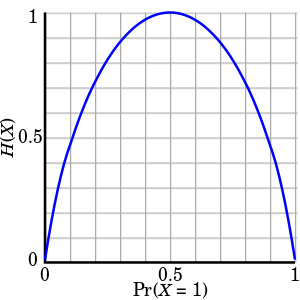
\includegraphics[scale=0.5]{img/entropy.png}
	\caption{Binary entropy function}
	\label{fig:entropy}
\end{figure}



The candidate functions, out of which the best on is chosen with the information gain, are \underline{randomly drawn}. Typically, one decides:
\begin{itemize}
    \item
        how many candidate functions are drawn
    \item
        if also linear projection of the data shall be drawn (e.g. consider only dimensions \(\{d_{i_1}, d_{i_2}, \dots, d_{i_n}\}\)
    \item
        how the splitting parameters are sampled
\end{itemize}
\(\Rightarrow\) Note that a sparser sampling leads to more "noise"/less optimal results. (\textit{Note:} might be desired, e.g. prevents overfitting)

Choice of tree depth:
\begin{itemize}
    \item
        set maximum depth ("mandatory")
    \item
        optional: set minimum number of samples for split 
    \item
        depending on the application, stop if for example 99\% of features in a node belong to one class
\end{itemize}

Final classifier output:
\begin{itemize}
    \item
        at a leaf node, report the relative frequencies of the class labels in that node (e.g., 15\%: class 1, 85\% class 2)
    \item
        combine al trees by averaging the individual tree outputs. If a single discrete label is required, decide for the class with maximum probability.
\end{itemize}

\section{Random Forests (continued)}
Example: Classification
\begin{enumerate}
    \item
        Randomly select a number of splitting functions 
    \item
        Evaluate the information gain for each splitting function
    \item
        Set the function with maximum information gain as the current nodes' decision function
    \item
        Recursively repeat for the child nodes, until max tree depth (or some other criterium) is reached 
\end{enumerate}

\subsection{Regression Forests}
Goal: predict a \underline{continous} label \(p(y|\vec{x})\). (Remark: choice of the model complexity is related to the bias/variance trade off)

"Leaf prediction model": a base function that is fitted to the samples. The leaf prediction model could be
\begin{multicols}{2}
\begin{itemize}
    \item
        constant
    \item
        linear
    \item
        polynomial
    \item
        ...
\end{itemize}
\end{multicols}

To faithfully represent all of the data with a single function, it would certainly make sense to use a polynomial model, or something even more complex. However, the random idea implies to subdivide/partition the space, and to fit simpler models to the individual partitions. As a specific example, let's split up our input data points:

\begin{figure}[ht]
	\centering
    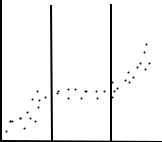
\includegraphics[height=4cm]{img/rf_regression.jpg}
	\caption{Regression split}
	\label{fig:rf_regression}
\end{figure}

The decision criterion for the splitting function works analogously to the classification case. The only difference ist that we need to define the entropy \(H(S_j)\) on continous values:
\[H(S_j) = -\frac{1}{\abs{S_j}} \cdot \sum_{\vec{x} \in S_j} \int_y p(y|x) \cdot log(y|x)dy\]
where \(p(y|x)\) can, e.g. be chosen as a Gaussian distribution \(p(y|x) = \mathcal{N}(y; \overline{y}(x), \sigma_y^2(x))\), where \(\overline{y}(x)\) is a linear function and \(\sigma_y(x)\) is the conditional variance computed from a linear fit.

%Probabilistic linear fit:
%\begin{figure}[H]
%	\centering
%    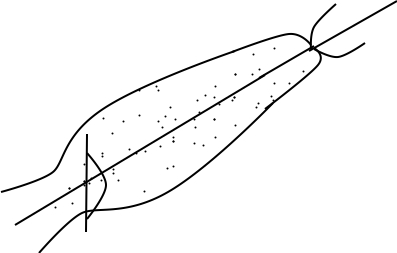
\includegraphics[height=4cm]{img/rf_linearfit.jpg}
%	\caption{Probabilistic linear fit}
%	\label{fig:rf_regression}
%\end{figure}

Combining the expression for \(p(y|x)\) into \(H(S_j)\) yields
\[H(S_j) = \frac{1}{\abs{S_j}} \cdot \sum_{\vec{x} \in S_j} \frac{1}{2} \cdot log((2 \pi e)^2 \sigma_y^2(\vec{x}))\]
\[\Rightarrow I(S_j, \vartheta) = \sum_{\vec{x} \in S_j} log(\sigma_y(\vec{x})) - \sum_{i \in \{L, R\}} (\sum_{x \in S_j^i} log (\sigma_y(\vec{x}))) \]

\subsection{Density Forests}
Very same idea, adapted to unlabelled data $\Rightarrow$ learning-baed density estimator.

Each leaf node is modeled as a multivariate Gaussian distribution. The information gain metric can again be reused, i.e. \(I(S_j, \vartheta) = H(S_j) - \sum_{i \in \{L, R\}} \frac{\abs{S_j^i}}{\abs{S_j}} \cdot H(S_j^i)\) but let us choose \(H(S_j)\) as
%Fancy
\[
H(S_j) = \frac{1}{2} \cdot log((2 \pi e)^d \abs{
    \underset{\mathllap{
        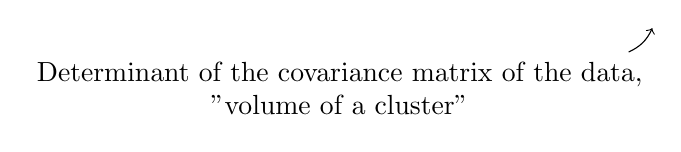
\begin{tikzpicture}
            \draw[->] (-0.3, 0) to[bend right=20] ++(0.3,2ex);
            \node[below left,align=center] at (0,0) {Determinant of the covariance matrix of the data,\\ "volume of a cluster"};
        \end{tikzpicture}
    }}{\Lambda} 
S_j})
\]

Plugging \(H(S_j)\) back into \(I(S_j, \vartheta)\) yields
\[I(S_j, \vartheta) = log (\abs{\Sigma(S_j)}) - \sum_{i \in \{L, R\}} \frac{\abs{S_j^i}}{\abs{S_j}} \cdot log(\abs{\Lambda(S_j^i)})\].

In each leaf, fit a multivariate Gaussian distribution to the data in that leaf using, e.g. MLE.

Note that the fitted densities have discontinuities at the splitting boundaries (this is the same type of discontinuity that we observed for regression forests or classification forests). However, remember that the result of a random forest is averaged over all individual trees. Because of randomization, each tree splits at a slightly different location, and thus the discontinuities are "averaged out" in the forest.


\section{Hidden Markov Models and Markov Random Fields}
Generative vs. Discriminative Model: let \(x\) denote the input, \(y\) the hidden variable/prediction/...
\[p(x,y) \Leftrightarrow p(y|x)\]

In a generative model, the available information is "more complete", i.e. we can for example also generate new samples \(x\) by sampling from \(p(x,y)\) by marginalizing over \(y\).

A discriminative model is slimmer (which is particularly useful for robust training with limited training data (the situation we're almost always in)); however, it only allows to discriminate between different \(y\)'s, but we can not generate new values \(x\).

\subsection{Remarks about HMMs}
\begin{itemize}
    \item
        Probabilistic, graphical model
    \item
        the directed edge in the graph can be understood as a statistical dependency: \[S_1 \rightarrow S_2 \Rightarrow p(S_2|S_1)\]
    \item
        Generative approach
    \item
        For many tasks, including speech processing, we oftentimes only allow for state transitions \(a_{ij}\) with \(i \leq j\). (no backward links) Those restricted HMMs are called "Left-right HMMs", as opposed to fully connected ("ergodic") HMMs.
\end{itemize}

\medbreak
How can we generate observations with an HMM?
\begin{enumerate}
    \item
        Sample from \(\pi = (\dots)\) (this gives you starting state) 
    \item
        Let \(S_1\) denote the starting state. Sample from \(b_1\) (column or row from production probability matrix \(B\)) a symbol
    \item
        Sample from \(\vec{a}_{S_1}\) (column or row from state transition matrix \(A\)) the next state
    \item
        Repeat 2.-3. until (randomly drawn/desired) word length reached
\end{enumerate}

\subsection{Markov Random Fields (MRF)}
1985, Geman/Geman: introduced MRFs to image processing:  Consider the pixel grid as a lattice (Gitter) of random variables.

More specifically, let us assume that the image \(F\) is given by the random matrix \([f_{ij}]\). %\(\Rightarrow p([f_{ij}])\). 

Assumption: limited statistical dependency:
\[p(f_{ij}| f_{i-1, j-1}, f_{i, j-1}, f_{i-1,j})\]
where \(f_{i-1, j-1}, f_{i, j-1}, f_{i-1,j})\) form a dependency of the neighbors to \(f_{i,j}\) (This will be our Markov property).

\[p([f_{ij}]) = \prod_{i,j} p(f_{i,j} | f_{i-1, j-1}, f_{i, j-1}, f_{i-1,j})\]

\subsubsection{Definition of MRF}
Lets us consider the features/observations \(\vec{x}_1,\vec{x}_2, \dots, \vec{x}_N\)
\begin{enumerate}
    \item
        Positivity: \(p(\vec{x}_1,\vec{x}_2, \dots, \vec{x}_N) > 0\)
    \item
        Markov property: \(p(\vec{x}_k | \vec{x}_1, \dots, \vec{x}_{k-1},\vec{x}_{k+1} \dots, \vec{x}_N) = p(\vec{x}_k|\mathcal{N}(\vec{x}_k))\) where \(\mathcal{N}(\vec{x}_k)\) denoted the neighborhood of \(\vec{x}_k\).
\end{enumerate}
Definition of the neighborhood: 
\begin{enumerate}
    \item
        \(\vec{x}_k \notin \mathcal{N}(\vec{x}_k)\)
    \item
        \(\vec{x}_i \in \mathcal{N}(\vec{x}_k) \Rightarrow \vec{x}_k \in \mathcal{N}(\vec{x}_i)\)
    \item
        \(\mathcal{N}(\vec{x}_k) = \{\vec{x}_i | 0 < dist(\vec{x}_i, \vec{x}_k) \leq t\}\)
\end{enumerate}
Example: Pixel grid:
\(\mathcal{N}(\vec{x}_{i,j}) = \{x_{k,l} | (i - k)^2 + (j - l)^2 \leq c^2, i \neq k \text{ or } j \neq l \}\)
\begin{itemize}
    \item
        NESW as neighbors, 4-Neighborhood \((c=1)\)
    \item
        All around as neighbors, 8-Neighborhood \((c=\sqrt 2)\)
\end{itemize}

\section{Markov Random Fields (continued)}
(Graph) clique: Complete subgraph

Gibbs Random Field (GRF): A GRF is given by the PDF 
\(p(x) = \frac{1}{
\underset{\mathllap{
        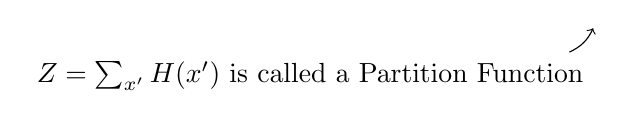
\begin{tikzpicture}
            \draw[->] (-0.3, 0) to[bend right=20] ++(0.3,2ex);
            \node[below left,align=center] at (0,0) {\(Z = \sum_{x'}H(x')\) is called a Partition Function};
        \end{tikzpicture}
    }}{Z}}  e^{-H(x)}\)
, where \(H(x)\) is an energy function, i.e. a sum of potential functions. For a given PDF \(p(x)\), the choice of energy function is not unique. Consider for example:
\[H(x) = - log p(x) - log Z \]
\[p(x) = \frac{1}{Z} e^{-H(x)} = \frac{1}{Z} e^{log p(x)} e^{log Z} = p(x)\]
\[\Rightarrow \text{we can chose Z arbitratily}\]

The interesting theoretical property is that GRF and MRF are equivalent. This is called the \textit{Hammersley-Clifford Theorem}.

\bigbreak

\subsection{Example: image denoising}
Given: Observed noisy image \([g_{ij}]\)

Hidden variables are the ideal (noiseless) images \([f_{ij}]\).

\textbf{Assumption 1:} the ideal image is spatially smooth \[p([f_{ij}]) = \frac{1}{Z} \cdot e^{-H([f_{ij}])}\] where \(H([f_{ij}]) = \sum_{ij} \norm{\Delta f_ij}_2^2\) (sum of squared gradients, computed over a neighborhood) (Note: Smoother image produces smaller \(H\), which maximizes \(p([f_{ij}])\).

\textbf{Assumption 2:} \([g_{ij}]\) is similar to \(f_{ij}\), but corrupted by additive Gaussian noise.
\[ p([g_{ij}]|[f_{ij}]) = \prod_{i,j} \frac{1}{\sqrt{2\pi} \sigma_{ij}} \cdot exp(-\frac{1}{2\sigma_{ij}^2} \cdot \underset{\text{energy function H}}{(f_{ij} - g_{ij})^2)}\]

With these two functions defined, we can solve for a MAP estimte for \(f\): 
\begin{align*}
    \underset{\text{estimated ideal image}}{[\hat{f}_{ij}]} &= \argmax_{[f_{ij}]} p([f_{ij}]|[g_{ij}])\\
    &= \argmax_{[f_{ij}]} p([g_{ij}]|[f_{ij}]) \cdot p([f_{ij}])\\
    &= \dots \text{(take log)}\\
    &= \argmin_{[f_{ij}]} \{\sum_{ij} \norm{\Delta f_{ij}}_2^2 + \sum_{ij} \lambda_{ij}(f_{ij} - g_{ij})^2\}
\end{align*}
\(\norm{\Delta f_{ij}}_2^2\): function of clique of size 2

Lecture slides: \url{https://www.slideshare.net/ykwang/markov-random-field-mrf} 

\section{Markov Random Fields}
\begin{figure}[ht]
	\centering
    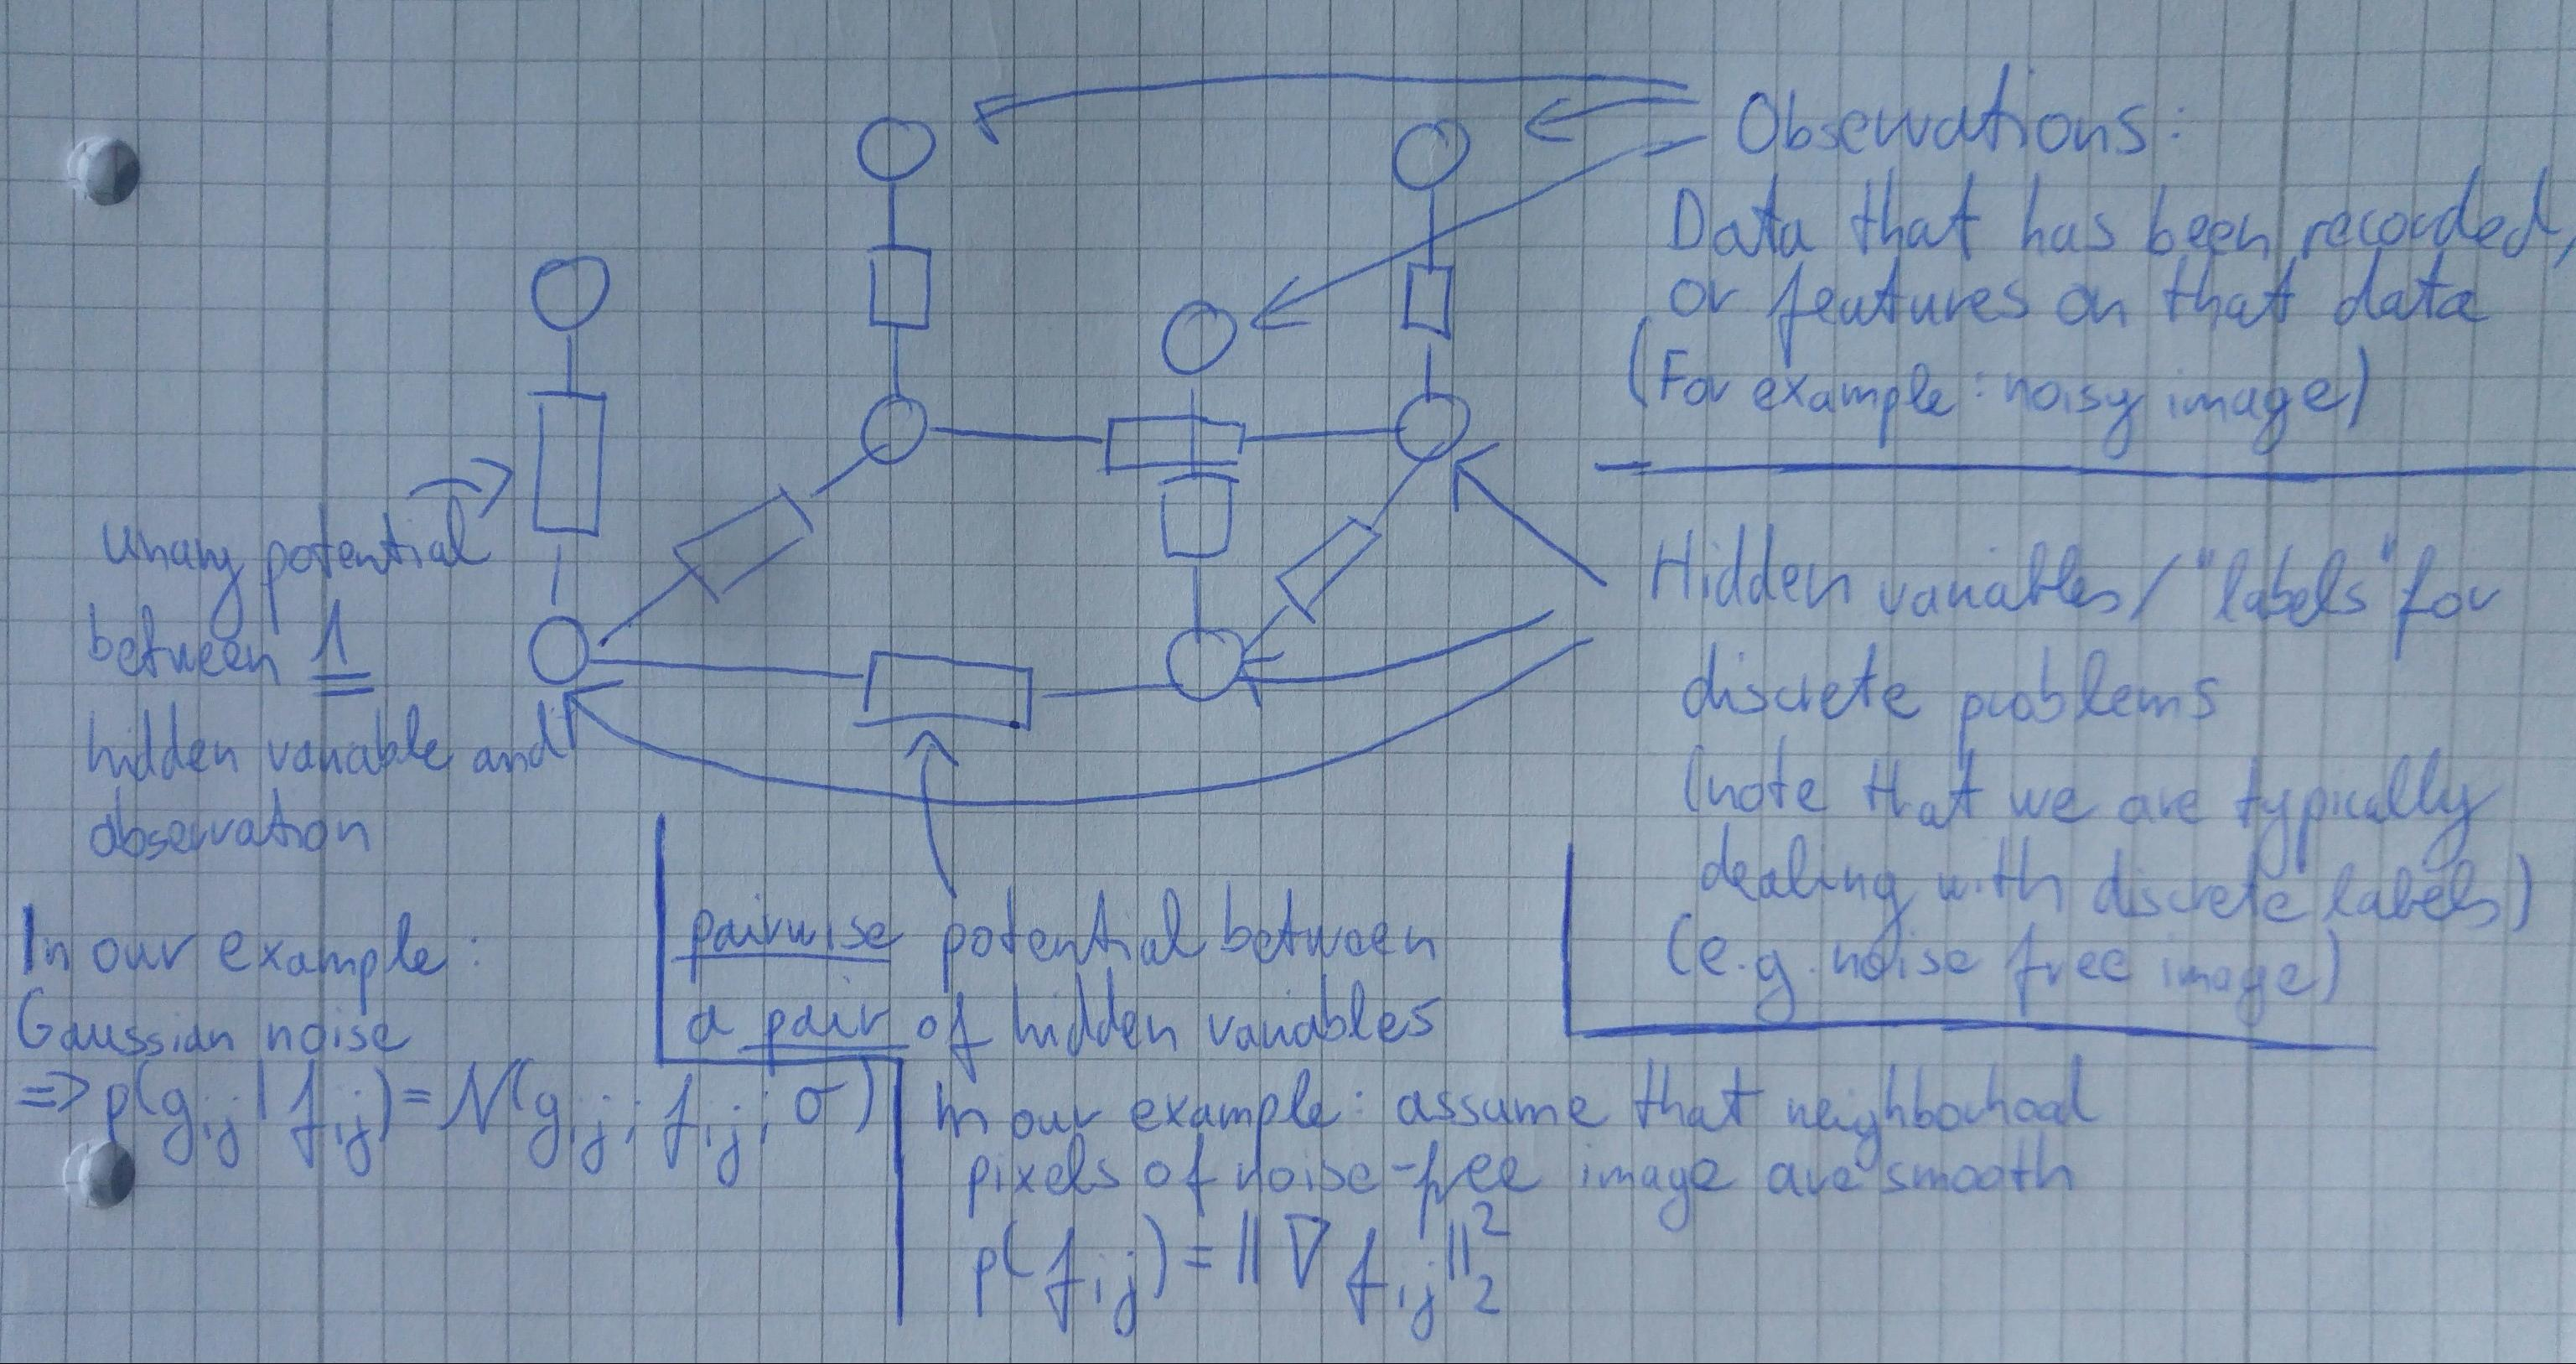
\includegraphics[scale=0.15]{img/mrf_1.jpg}
	\caption{MRF for image denoising}
	\label{fig:mrf_1}
\end{figure}

From a engineering perspective, we model the hidden variables by defining the unary and pairwise potentials. These are local relationships in the graph, i.e. they don't require complicated non-local interactions to be considered.

Remember from last week: a MRF and a GRF (Gibbs Random Field) are equivalent (\textit{Hammersley-Clifford} theorem).
This means that we can exchange the probabilities (defining the PDFs between the nodes in the MRF model might be impossible/hard) that describe the node relationships by potentials.

\[p(\vec{x}) = \prod_C p_C(\vec{x}_C) = \frac{1}{Z} \prod_C \psi_C(x_C)\]

Such potentials are much easier to design: We are typically interested in potential functions that assume a minimum value in a specific situation, e.g. \(\norm{\Delta f_{ij}}_2^2\) is minimal if \(f_{i,j} = f_{i,j+1} = \dots\), that depends on what we would like to achieve with the MRF.

\(p(x_1, \dots, x_N) = \prod \dots\) independent segments of the random variables \(x_1, \dots, x_N\)

General form of a Gibbs potential:
\begin{align*}
    p(\vec{x}) &= \frac{1}{Z} \prod_C \phi_C (\vec{x}_C)
    = \frac{1}{Z} \prod_C e^{-H(\vec{x}_C)}
    = \frac{1}{Z} e^{- \sum_C H(\vec{x}_C)}
\end{align*}
where \(H(\vec{x}_C) = \norm{\Delta f_{ij}}_2^2\) or \(H(\vec{x}_C) = \mathcal{N}(g_{ij}, f_{ij}, \sigma))\).

\bigskip

\(H(\vec{x}_C)\) is an energy function that is defined over clique potentials. Solvers for Markov Random Fields seek to directly minimize \(H(\vec{x}_C)\) instead of maximizing \(\psi_C(x_C)\).

A modern way of solving an MRF is via \underline{graph cuts}\footnote{ Kolmogorov, Zabih: "What Energy Functions Can Be Minimized via Graph Cuts?"}.

\subsection{Maximum Flow and Minimum Cut}
\begin{figure}[ht]
	\centering
    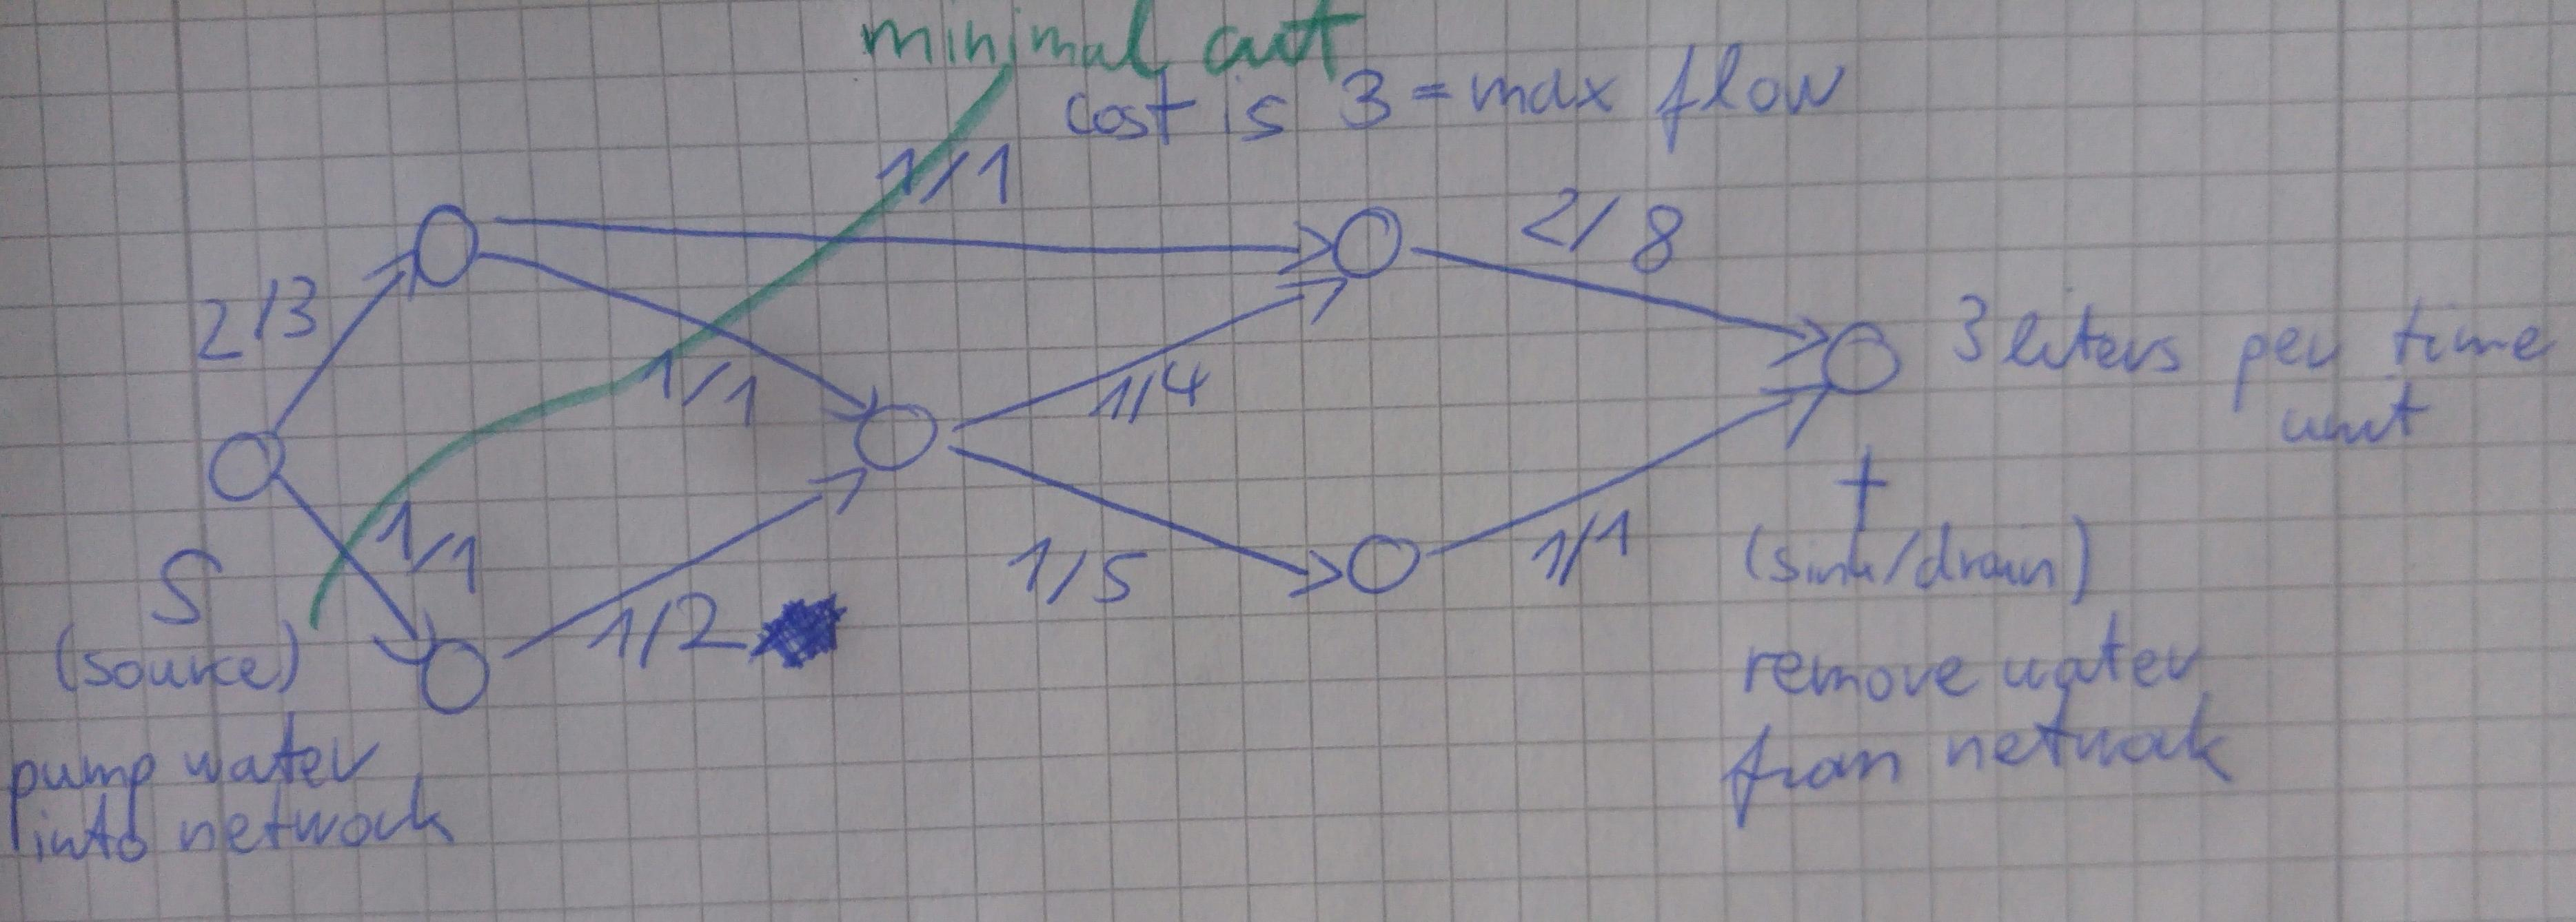
\includegraphics[scale=0.13]{img/mrf_2.jpg}
	\caption{Max Flow Min Cut}
	\label{fig:mrf_2}
\end{figure}

There are a number of classic algorithm that solve the max flow problem in polynomial time.

A minimum cut divides a network into two parts \(s, t\), such that the sum of the edge weights that are cut are minimal.

A solution to the maximum flow problem is a solution to the minimum cut problem: the minimum cut consists of edges that are fully used in the solution to the max flow problem.

\newpage
\begin{appendices}

\section{Lawrence R. Rabiner, Fellow: A Tutorial on Hidden Markov Models and Selected Applications in Speech Recognition}
\subsection{Discrete Markov Processes}
\begin{itemize}
    \item
        set of \(N\) discrete states \(S_1, S_2, \dots, S_N\)
    \item
        set of state transition probabilities \(a_{ij} = P(q_t = S_j | q_{t-1}=S_i)\)
%    \item
%        First order Markov chain: \(P(q_t = S_j|q_{t-1} = S_i, q_{t-2} = S_k, \dots) = P(q_t = S_j | q_{t-1}=S_i)\).
    \item
        properties: \(a_{ij} \geq = 0\) and \(\sum_{j=1}^N a_{ij} = 1\)
    \item
        the states itself are observable
    \item
        Calculating the probability of observations sequence given a model:
        \begin{align*}
            P(O|Model) &= P(S_3, S_3, S_1, S_1, S_3, S_2, S_3|Model)\\
            &= P(S_3) \cdot P(S_3|S_3) \dots P(S_3|S_2)\\
            &= \pi_3 \cdot a_{33} \dots a_{23}\\
            &= \dots
        \end{align*}
        where \(\pi_i = P(q_1 = S_i)\) is the initial state probability
\end{itemize}

\subsection{Extension to Hidden Markov Models}



\section[Undirected Graphical Models]{Undirected Graphical Models (Markov Random Fields) \protect\footnote{The Elements of Statistical Learning: Chapter 17, Undirected Graphical Models}}
\subsection{Introduction}
\begin{itemize}
    \item
        Consist of vertices (nodes) and edges joining some pairs of vertices
    \item
        Each vertex represents a random variable
    \item
        No edge between two vertices \(\Rightarrow\) conditionally independent, given the other variables
    \item
        Edges are parameterized by values or \textit{potentials} that encode the strength of the conditional dependence between the random variables
    \item
        Main challenges: model selection (structure), estimation of edge parameters from data (learning), and computation of marginal vertex probabilities and expectations, from their joint distribution (inference)
\end{itemize}

\subsection{Markov Graphs and Their Properties}
A graph \(\mathcal{G}\) consists of a pair \((V,E)\), where \(V\) is a set of vertices and \(E\) the set of edges (defined by pairs of vertices). Two vertices \(X\) and \(Y\) are called adjacent if there is a edge joining them; this is denoted by \(X \sim Y\). A \textit{complete graph} is a graph with every pair of vertices joined by an edge.

In a Markov graph \(\mathcal{G}\), the absence of an edge implies that the corresponding random variables are conditionally independent given the variables at the other vertices (known as \textit{pairwise Markov independencies} of \(\mathcal{G}\)). Notation:
\[\text{No edge joining } X \text{ and } Y \Leftrightarrow X \bot Y | \text{rest} \]
If \(A,B\) and \(C\) are subgraphs, then \(C\) is said to \textit{separate} \(A\) and \(B\) if every path between \(A\) and \(B\) intersects a node in \(C\). Separators have the nice property that they break the graph into conditionally independent pieces (known as \textit{global Markov properties} of \(\mathcal{G}\)). Notation:
\[\text{if } C \text{ separates } A \text{ and } B \text{ then } A \bot B |C\]

Pairwise and global Markov properties of a graph are equivalent. This is, the set of graphs with associated probability distributions that satisfy the pairwise Markov independencies and global Markov assumptions are the same. This is useful for inferring global independence relations from simple pairwise properties.

The global Markov property allows us to decompose graphs into smaller more manageable pieces and thus leads to essential simplifications in computation and interpretation. A \textit{clique} is a complete subgraph - a set of vertices that are all adjacent to one another (\textit{maximal} if no other vertices can be added to it).

A probability density function \(f\) over an Markov graph \(\mathcal{G}\) can be represented as
\[f(x) = \frac{1}{Z} \prod_{C \in \mathcal{C}} \psi_C(x_C)\]
where \(\mathcal{C}\) is the set of maximal cliques, and the postitive functions \(\psi_C(\cdot)\) are called \textit{clique potentials}. These are not in general density function, but rather are affinities that capture the dependence in \(X_c\) by scoring certain instances \(x_c\) higher than other. The quantity
\[Z = \sum_{x \in \mathcal{X}}\prod_{C \in \mathcal{C}} \psi_C (x_C)\]
is the normalizing constant, also known as \textit{partition} function.

This definition of \(f\) implies a graph with independence properties defined by the cliques in the product. This holds for Markov networks \(\mathcal{G}\) with positive distributions, and is known as the \textit{Hammersley-Clifford} theorem.

Because we are restricted to potential functions which are stritly positive it is convenient to express them as exponentials, so that
\[\psi_C(x_C) = exp(-E(x_C))\]
where \(E(x_C)\) is called an \textit{energy function}, and the exponential representation is called the \textit{Boltzmann distribution}. The joint distribution is defined as the product of potentials, and so the total energy is obtained by adding the energies of each of the maximal cliques.

\subsection{Image de-noising \protect\footnote{Bishop, Pattern Recognition: 8.3.3}}
Let the observed noisy image be described by an array of binary pixel values \(y_i \in \{-1, +1\}\), where the index \(i = 1, \dots, D\) runs over all pixels. We shall suppose that the image is obtained by taking  an unknown noise-free image, described by binary pixel values \(x_i \in \{-1, +1\}\) and randomly flipping the sign of pixels with some small probability.

Because the noise level is small, we know that there will be a strong correlation between \(x_i\) and \(y_i\). We also know that neighbouring pixels \(x_i\) and \(x_j\) in an image are strongly correlated.

\underline{TODO:} Random field model picture

This graph has two types of cliques, each of which contains two variables. The cliques \(\{x_i, y_i\}\) have an associated energy function that expresses the correlation between these variables (\(-\eta x_i y_i)\), where \(\eta\) is a positive constant) \(\Rightarrow\) lower energy (higher probability) when \(x_i\) and \(y_i\) have the same sign.

The remaining cliques comprise pairs of variables \(\{x_i, x_j\}\) where \(i, j\) are indices of neighbouring pixels. Again, we want the energy to be lower when the pixels have the same sign than when they have the opposite sign, and so we choose an energy given by \(-\beta x_i x_j\), where \(\beta\) is a positive constant.

Additionally, we add a term \(hx_i\) for each pixel \(i\) in the noise-free image. Such a term has the effect of biasing the model towards pixel values that have one particular sign in preference to the other.

The complete energy function for the model then takes the form
\[E(x,y) = h \sum_i x_i - \beta \sum{\{i,j\}} x_ix_j - \eta \sum_i x_i y_i\]
which defines a joint distribution over \(x\) and \(y\) given by
\[p(x,y) = \frac{1}{Z} exp\{-E(x,y)\}\]

\underline{\textit{Note:}}
\begin{align*}
    f(x) &= \frac{1}{Z} \prod_{C \in \mathbb{C}} \psi_C(x_C)\\
    &= \frac{1}{Z} \prod_{C \in \mathbb{C}} exp\{-E(x_C)\}\\
    &= \frac{1}{Z} exp\{-\sum_{C \in \mathbb{C}}E(x_C)\}
\end{align*}

We now fix the elements of \(y\) to the observed values given by the pixels of the noisy image, which implicitly defines a conditional distribution \(p(x|y)\) over noise-free images (see lecture).

\end{appendices}
\end{document}
